%%%%%%%%%%%%%%%%%%%%%%%%%%%%%%%%%%%%%%%%%%%%%%%%%%%%%%%%%%%%%%%%%%%%%%%%%%%%%%%%
%2345678901234567890123456789012345678901234567890123456789012345678901234567890
%        1         2         3         4         5         6         7         8

%\documentclass[letterpaper, 10 pt, conference]{ieeeconf}  % Comment this line out
                                                          % if you need a4paper
\documentclass[a4paper, 10pt, conference]{ieeeconf}      % Use this line for a4
                                                          % paper
\IEEEoverridecommandlockouts                              % This command is only
                                                          % needed if you want to
                                                          % use the \thanks command
\overrideIEEEmargins
% See the \addtolength command later in the file to balance the column lengths
% on the last page of the document

\usepackage{graphicx}
\usepackage{graphics}

% The following packages can be found on http:\\www.ctan.org
%\usepackage{graphics} % for pdf, bitmapped graphics files
%\usepackage{epsfig} % for postscript graphics files
%\usepackage{mathptmx} % assumes new font selection scheme installed
%\usepackage{times} % assumes new font selection scheme installed
%\usepackage{amsmath} % assumes amsmath package installed
%\usepackage{amssymb}  % assumes amsmath package installed

\title{\LARGE \bf
Preparación del Informe para IPyAN
}

%\author{ \parbox{3 in}{\centering Huibert Kwakernaak*
%         \thanks{*Use the $\backslash$thanks command to put information here}\\
%         Faculty of Electrical Engineering, Mathematics and Computer Science\\
%         University of Twente\\
%         7500 AE Enschede, The Netherlands\\
%         {\tt\small h.kwakernaak@autsubmit.com}}
%         \hspace*{ 0.5 in}
%         \parbox{3 in}{ \centering Pradeep Misra**
%         \thanks{**The footnote marks may be inserted manually}\\
%        Department of Electrical Engineering \\
%         Wright State University\\
%         Dayton, OH 45435, USA\\
%         {\tt\small pmisra@cs.wright.edu}}
%}

\author{G. Brunini, V. Catacora y L. Reb\'on\\ %\vspace{1cm}
{\it Introducción a la Programacióon y Análisis Numerico, Depto. de Ciencias B\'asicas}\\  {\it Facultad de Ingenier\'ia, UNLP, La Plata, Argentina.}}                                            % <-this % stops a space

\begin{document}

\maketitle
\thispagestyle{empty}
\pagestyle{empty}


%%%%%%%%%%%%%%%%%%%%%%%%%%%%%%%%%%%%%%%%%%%%%%%%%%%%%%%%%%%%%%%%%%%%%%%%%%%%%%%%
\begin{abstract}

Estas instrucciones son una gu\'ia b\'asica para la preparaci\'on del informe a presentar y un ejemplo del formato deseado que puede ser usado como plantilla.

El Resumen debe enunciar concisamente que fue hecho, como fue hecho, resultados principales, y su trascendencia. No debe contener ecuaciones, figuras, tablas, o referencias. 


\end{abstract}


%%%%%%%%%%%%%%%%%%%%%%%%%%%%%%%%%%%%%%%%%%%%%%%%%%%%%%%%%%%%%%%%%%%%%%%%%%%%%%%%
\section{INTRODUCCCI\'ON}

El formato de esta plantilla sigue el est\'andar de la IEEE\footnote{Institute of Electrical and Electronics Engineers.}.  La longitud de las secciones no guarda ninguna relaci\'on con lo que se espera del informe.

En la introducci\'on explicar claramente cu\'al es el problema a abordar, c\'omo se lo pretende estudiar, que es lo que se va a hacer, las motivaciones, etc.

Recordar siempre citar los trabajos, libros y todo material bibliogr\'afico al que se hace referencia en el texto, o de los cuales se sac\'o informaci\'on/modelos/texto para el presente trabajo. No copie p\'arrafos de otros informes, trabajos, libros, p\'aginas web, etc. Si fuera necesaria alguna cita textual, adem\'as de referenciarse debe incluirse como texto entre comillas.


\section{MARCO TE\'ORICO}

Explicar los modelos te\'oricos a ser utilizados para contrastar/ajustar a los datos o mediciones. Ac\'a van las ecuaciones, sus resoluciones y justificaciones de los modelos a utilizar. Se deben incorporar las referencias bibliogr\'aficas utilizadas y/o consultadas que dan soporte a lo que aqu\'i se desarrolla.

\subsection{Preparaci\'on del informe}

Esta plantilla corresponde a un formato A4 (210 por 297 mm), hoja completa. Los m\'argenes para la hoja est\'an definidos para ser: superior = 19 mm, inferior = 30 mm, lado = 13 mm. El ancho de la columna es de 88 mm.  El espacio entre las dos columnas es de 4 mm.  La sangr\'ia al inicio de cada p\'arrafo es de 3,6 mm.
El texto en las columnas debe estar justificado. El ancho de las figuras y tablas debe ajustarse, preferentemente, al de la columna.

\subsection{Tama\~no y tipo de fuente}
Se pueden seguir los tama\~nos especificados en esta plantilla. Como una ayuda para determinar el tama\~no de la letra, 1 punto corresponde a 0,35 mm.  Time New Roman es la fuente preferida. Prestar especial atenci\'on al tama\~no y tipo de fuente que utiliza en las figuras para que sea legible en la versión impresa. 

\subsection{Referencias}

Los n\'umeros de las citas deben ser consecutivos y entre corchetes \cite{c1}. Para remitirse en el texto a una referencia, use Ref.~\cite{c3}: ``El trabajo de la Ref.~\cite{c3} fue el primero en enunciar este postulado...", o ``...como se expone en las Refs.~\cite{c1,c5}", o ``Varios autores coinciden en este primer punto \cite{c1,c2,c3,c4}.", seg\'un sea el caso. 

Enumere las {\it notas al pie} separadamente con un super\'indice. Coloque la nota al pie en el inferior de la misma columna en que es citada.  No ponga las notas al pie en la lista de referencias.  

Dar los nombres de todos los autores; usar ``et al." si hay seis autores o m\'as.  Los trabajos que no han sido publicados, incluso si ellos han sido presentados para publicaci\'on, deben ser citados como ``no publicado"~\cite{c4}.  Los trabajos que han sido aceptados para publicaci\'on deben ser citados como ``en prensa" ~\cite{c5}.  Tambi\'en debe citarse el material que se extraiga de p\'aginas web ~\cite{c8}.

\subsection{Ejemplo del uso de Referencias}

El polinomio \'unico $p(x)$ de grado $\leq n$ que interpola un conjunto de $n+1$ puntos puede obtenerse, por ejemplo, a partir del c\'alculo de los polinomios de Lagrange \cite{c6}. Dado que este polinomio es \'unico, el error de truncamiento cometido al aproximar una funci\'on $f(x)$ por el polinomio interpolante en la forma de Lagrange ser\'a el mismo que al hacerlo mediante el polinomio interpolante en la forma de Newton. La demostraci\'on para puede encontrarse en la Ref.~\cite{c7}.

\section{SOLUCIONES NUM\'eRICAS}

Describir la metodolog\'ia utilizada para la resoluci\'on de cada uno de los problemas, qu\'e algoritmos se utilizaron, c\'omo fueron desarrollados, en qu\'e lenguaje, qu\'e problemas permiten resolver, bajo qu\'e condiciones, etc. Si fuera necesario, puede apoyarse de la utilizaci\'on de gr\'aficos y/o esquemas, o puede ser de utilidad copiar algunas l\'ineas del c\'odigo al momento de explicar alg\'un desarrollo particular.

Citar los archivos .m utilizados ya que estos deber\'an ser entregados para su correcci\'on.


\section{RESULTADOS Y DISCUCI\'ON}

Describir aqu\'i los resultados obtenidos a partir de la soluci\'on num\'erica y/o anal\'itica de cada problema. Se discutir\'an las limitaciones de cada modelo, ventajas y desventajas de los m\'etodos y algoritmos utilizados, comparando unos con otros en caso de ser pertinente, y entre estos y las soluciones anal\'iticas. Analizar el tipo y magnitud de los errores, sacar conclusiones al respecto, etc. Usar gr\'aficos y/o tablas dependiendo del tipo de resultado que se quiere mostrar y referenciarlas.

%%%%%%%%%%%%%%%%Tabla simple
\begin{table}[h]
\begin{center}
\begin{tabular}{|c||c|}
\hline
Propiedad & Valor\\
\hline
Corriente [A]& 4.9\\
\hline
Voltaje [V]& 218\\
\hline
\end{tabular}
\end{center}
\caption{Descripci\'on de la Tabla}
\label{tab:simple}
\end{table}

En el texto principal se har\'a referencia a cada una de las tablas explicando su contenido. La Tabla \ref{tab:simple} muestra un ejemplo de tabla simple generada en LaTeX, en tanto la Tabla \ref{tab:compleja} es un ejemplo m\'as complejo que une celdas de varias filas y columnas. 

%%%%%%%%%%%%%%%%Tabla compleja
\begin{table}[!h]
\begin{center}
\begin{tabular}{|l|c|c|}
\cline{2-3}
\multicolumn{1}{c}{}& \multicolumn{2}{|c|}{Datos} \\
\cline{2-3}
\multicolumn{1}{c|}{}& Propiedad & Valor \\
\hline \cline{2-3} {$t_1$} & Corriente  & 5.3 A \\
\cline{2-3}
                      & Voltaje    & 220 V\\
\hline \cline{2-3} {$t_2$} & Corriente  & 4.9 A \\ \cline{2-3}
                     & Voltaje    & 218 V\\
\hline
 \end{tabular}
 \end{center}
 \caption{Valores observados de corriente y voltaje en distintos instantes de tiempo $t_i$.}
 \label{tab:compleja}
\end{table}


%%%%% Figure
\begin{figure}[htp]
\centering
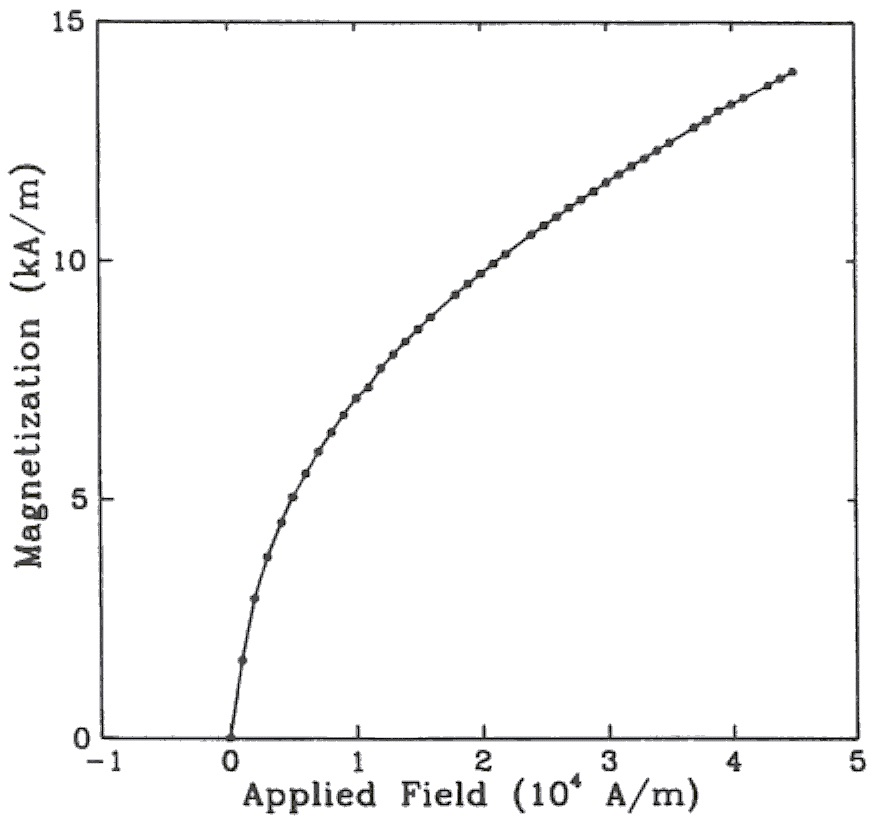
\includegraphics[width=0.43\textwidth]{./figuras/Fig.jpg}
\caption{Magnetizaci\'on como funci\'on del campo aplicado.
Note que la leyenda de la figura est\'a centrada en la columna. } 
\label{fig:fig}
\end{figure}

Como ejemplo de formato para las figuras podemos ver la Fig.\ref{fig:fig} en donde se obserba el valor de magnetizaci\'on en funci\'on del campo magn\'etico aplicado. Los puntos representan los valores obtenidos experimentalmente en tanto que la l\'inea continua se corresponde con el ajuste realizado para tal conjunto de puntos.  

\section{CONCLUCIONES}

Dependiendo de las caracter\'isticas del trabajo, de los datos analizados o del sistema estudiado las discusiones pueden presentarse en una secci\'on final o incluirse en la presentaci\'on de los resultados. No es una secci\'on estrictamente requerida. Aunque puede ser \'util como un repaso de los puntos m\'as importantes del trabajo, no debe ser una replica del Resumen. Debe elaborarse para destacar la importancia del trabajo realizado presentado, para sugerir cambios, mejoras, aplicaciones o extenciones futuras.
 

\addtolength{\textheight}{-12cm}   % This command serves to balance the column lengths
                                  % on the last page of the document manually. It shortens
                                  % the textheight of the last page by a suitable amount.
                                  % This command does not take effect until the next page
                                  % so it should come on the page before the last. Make
                                  % sure that you do not shorten the textheight too much.

%%%%%%%%%%%%%%%%%%%%%%%%%%%%%%%%%%%%%%%%%%%%%%%%%%%%%%%%%%%%%%%%%%%%%%%%%%%%%%%%



%%%%%%%%%%%%%%%%%%%%%%%%%%%%%%%%%%%%%%%%%%%%%%%%%%%%%%%%%%%%%%%%%%%%%%%%%%%%%%%%



%%%%%%%%%%%%%%%%%%%%%%%%%%%%%%%%%%%%%%%%%%%%%%%%%%%%%%%%%%%%%%%%%%%%%%%%%%%%%%%%
\section*{Ap\'endice}


\section*{A.  ALGUNAS CONVENCIONES SOBRE FORMATO}

En esta secci\'on se describen en m\'as detalle algunas convenciones sobre el formato del informe en general.

\subsection*{A.1     Lenguaje}

Es sumamente importante entender que un trabajo cien\-t\'ifico o un informe t\'ecnico debe tener un tenor objetivo y formal, por lo tanto se recomienda evitar apreciaciones subjetivas y expresiones coloquiales en el mismo. Tenga en cuenta que el sentido de ciertas palabras o expresiones en el lenguaje coloquial puede ser completamente distinto al que tiene tienen t\'ecnicamente. 

Preste atenci\'on a la redacci\'on del texto; no es s\'olo una cuesti\'on de formalidad del lenguaje, sino fundamentalmente de presentar un trabajo que sea claro y entendible, sin renunciar a la rigurosidad de lo que se expone. En este sentido, es fundamental una gram\'atica correcta. As\'i mismo, los errores ortogr\'aficos restan claridad y seriedad a cualquier trabajo. La omisi\'on del acento escrito o la mala utilizaci\'on de los mismos es un error ortogr\'afico grave. Revise y corrija su trabajo antes de presentarlo.

\subsection*{A.2		Ecuaciones}

Las ecuaciones deben ser tratadas como parte de una oraci\'on (estando o no en l\'inea), es decir, deben est\'a seguidas de punto, coma, etc, como en
\begin{equation}
     a + b = c.
\end{equation}\label{ec:ejemplo}

Para los s\'imbolos, utilice It\'alicas. Todas las variables y par\'ametros involucrados en la ecuaci\'on deben estar definidos en el texto antes de que la misma sea presentada o inmediatamente despu\'es. Enumere las ecuaciones consecutivamente con el n\'umero de ecuaci\'on entre par\'entesis al mismo nivel en el margen derecho, como en la Ec.~(1). La ecuaci\'on se referencia en el texto como Ec.~(1), Ecs.~(1) y (2), etc., excepto en el comienzo de una oraci\'on: ``La ecuaci\'on (1) es...", ``...como se desprende de la Ec.~(1)."


 \subsection*{A.3		Figuras y Tablas}

A diferencia de las ecuaciones, las figuras y tablas no se consideran parte del texto. Pueden flotar sobre el texto y ser acomodadas donde mejor queden despu\'es de que son referenciadas en el texto. La forma de referenciarlas es escribiendo Fig. 1, Figs. 1, Fig. 1 (a) o Tabla I, seg\'un sea el caso. Todas las figuras y tablas deben estar referenciadas en el texto en donde se har\'a una discusi\'on de lo que se esquematiza en las mismas o los resultados que se presentan. 

Deben tener una resoluci\'on 'aceptable' como para poder apreciarse lo que se quiere mostrar. En el caso de gr\'aficos, los ejes deben est\'a claramente identificados con sus correspondientes unidades; los caracteres, tanto letras como n\'umeros, deben ser legibles (considere alrededor de un tama\~no 10). Para cada figura/subfigura o tabla se incluir\'a debajo de la misma una leyenda clara, concisa y autoexplicativa de lo que se est\'a mostrando. Las figuras y tablas grandes pueden expandirse abarcando ambas columnas.  

Las etiquetas de los ejes de las figuras son frecuentemente una fuente de confusi\'on.  Use palabras en vez de s\'imbolos. Por ejemplo, escriba ``Magnetizaci\'on" o ``Magnetizaci\'on (M)" no s\'olo ``M".  Ponga las unidades en par\'entesis.  No etiquete los ejes solo con las unidades.  En el ejemplo, se escribi\'o ``Magnetizaci\'on (A/m)" o ``Magnetizaci\'on (A*m$^{-1}$)".  

\section*{B.  OTRAS RECOMENDACIONES}
 
\subsection*{B.1		Unidades}

Al trabajar con modelos que describen una situaci\'on real (no son s\'olo un problema matem\'atico) se deben incluir las unidades de las magnitudes. Enuncie claramente las unidades para cada cantidad que use en una ecuaci\'on, tablas, figuras, etc. Las unidades SI (MKS) son las recomendadas.

Evite combinar unidades de sistemas distintos Esto frecuentemente lleva a confusi\'on a causa de que la ecuaci\'on no est\'a balanceada en sus magnitudes. 

\subsection*{B.2		Abreviaciones y Acr\'onimos}

Defina las abreviaciones y acr\'onimos en la primera vez que son usados en el texto, incluso si ellos han sido definidos en el abstract, por ejemplo ``La forma de resolver una ecuaci\'on diferencial ordinaria (EDO)..."; una vez definida podr\'a usar las siglas en el resto.  Abreviaciones com\'unmente usadas tales como IEEE, SI, MKS, CGS, ac, dc y rms no tienen que ser definidas.  No use abreviaciones en el t\'itulo a menos que sea inevitable.


%\section*{ACKNOWLEDGMENT}

%The preferred spelling of the word Òacknowledgment\'o in America is without an Òe\'o after the Òg\'o. Avoid the stilted expression, ÒOne of us (R. B. G.) thanks . . .\'o  Instead, try ÒR. B. G. thanks\'o. Put sponsor acknowledgments in the unnumbered footnote on the first page.



%%%%%%%%%%%%%%%%%%%%%%%%%%%%%%%%%%%%%%%%%%%%%%%%%%%%%%%%%%%%%%%%%%%%%%%%%%%%%%%%


\begin{thebibliography}{99}

\bibitem{c1}	G. Eason, B. Noble, and I.N. Sneddon, ``On certain integrals of Lipschitz-Hankel type involving products of Bessel functions,” Phil. Trans. Roy. Soc. London, vol. A247, pp. 529-551, April 1955. 
\bibitem{c2}	J. Clerk Maxwell, A Treatise on Electricity and Magnetism, 3rd ed., vol. 2. Oxford: Clarendon, 1892, pp.68-73.
\bibitem{c3}	I.S. Jacobs and C.P. Bean, ``Fine particles, thin films and exchange anisotropy,” in Magnetism, vol. III, G.T. Rado and H. Suhl, Eds. New York: Academic, 1963, pp. 271-350.
\bibitem{c4}	K. Elissa, ``Title of paper if known,” no puplicado.
\bibitem{c5}	R. Nicole, ``Title of paper with only first word capitalized,” J. Name Stand. Abbrev., en prensa. 
\bibitem{c6}	Lloyd N. Trefethen and David Bau III, ``Numerical Linear Algebra” (Society for Industrial and Applied Mathematics, Philadelphia, UK, 1997).
\bibitem{c7}	E. Isaacson and H. B. Keller, ``Analysis of Numerical Methods”, Dover Publication, Inc. New York, Cap.5, Pag. 190. 1er Ed. (1996).
\bibitem{c8}    Argosy Medical Animation. (2007-2009). Visible body: anatomy. New York, EU.: Argosy Publishing. http://www.visiblebody.com (visitado el d\'ia 5/5/2019)

\end{thebibliography}




\end{document}
